% This file was created by tikzplotlib v0.9.8.
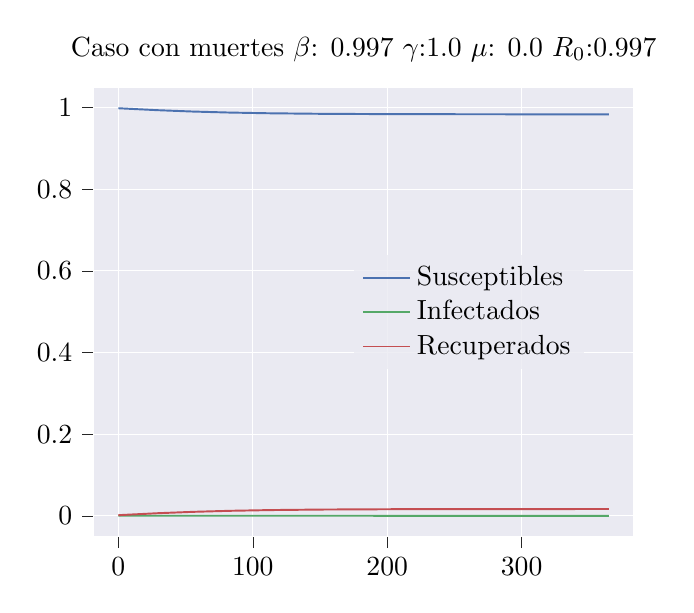
\begin{tikzpicture}

\definecolor{color0}{rgb}{0.917647058823529,0.917647058823529,0.949019607843137}
\definecolor{color1}{rgb}{0.298039215686275,0.447058823529412,0.690196078431373}
\definecolor{color2}{rgb}{0.333333333333333,0.658823529411765,0.407843137254902}
\definecolor{color3}{rgb}{0.768627450980392,0.305882352941176,0.32156862745098}

\begin{axis}[
axis background/.style={fill=color0},
axis line style={white},
legend cell align={left},
legend style={
  fill opacity=0.8,
  draw opacity=1,
  text opacity=1,
  at={(0.91,0.5)},
  anchor=east,
  draw=none,
  fill=color0
},
tick align=outside,
tick pos=left,
title={Caso con muertes
\(\displaystyle \beta\): 0.997 \(\displaystyle \gamma\):1.0 \(\displaystyle \mu\): 0.0 \(\displaystyle R_0\):0.997},
x grid style={white},
xmajorgrids,
xmin=-18.25, xmax=383.25,
xtick style={color=white!15!black},
y grid style={white},
ymajorgrids,
ymin=-0.0499110902972906, ymax=1.04814213104607,
ytick style={color=white!15!black}
]
\addplot [line width=0.7pt, color1]
table {%
0 0.998230695724487
29.0796699523926 0.993506193161011
55.1511001586914 0.99019730091095
82.2252731323242 0.987723827362061
112.307693481445 0.985923886299133
150.412094116211 0.984624743461609
203.557693481445 0.983811140060425
299.821441650391 0.983413696289062
365 0.983360052108765
};
\addlegendentry{Susceptibles}
\addplot [line width=0.7pt, color2]
table {%
0 0.000178217887878418
365 4.76837158203125e-07
};
\addlegendentry{Infectados}
\addplot [line width=0.7pt, color3]
table {%
0 0.00159108638763428
30.0824184417725 0.00649344921112061
56.1538467407227 0.00980234146118164
83.2280197143555 0.0122758150100708
113.310440063477 0.0140758752822876
151.414840698242 0.0153751373291016
204.560440063477 0.0161887407302856
299.821441650391 0.0165848731994629
365 0.0166394710540771
};
\addlegendentry{Recuperados}
\end{axis}

\end{tikzpicture}
